% Tabela: Resultados do Experimento Omega
\begin{table}[H]
	\centering
	\caption{Tabela de resultados do Experimento 4.}
		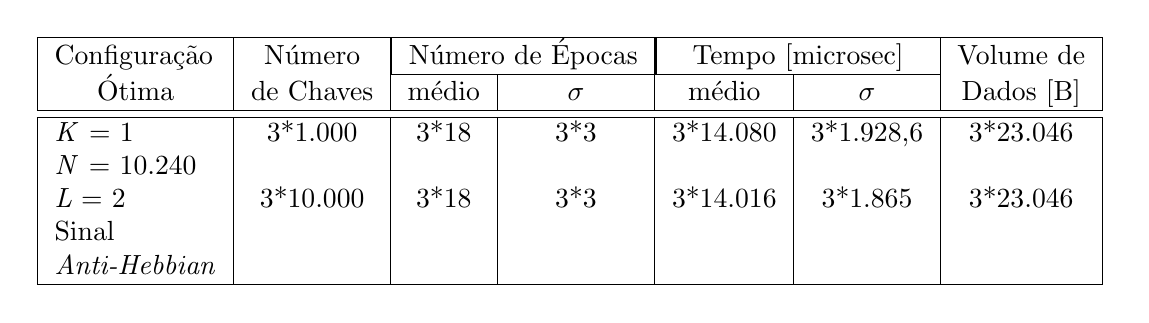
\begin{tikzpicture}
			
		\node[thick, align=center] (table) {
			\begin{tabular}{ |l|c|c|c|c|c|c| }
				\hline
				% \multicolumn{7}{ |c| }{Resultados do Experimento 4} \\
				% \hline \hline
				Configuração &
				Número &
				\multicolumn{2}{ |c| }{Número de Épocas} &
				\multicolumn{2}{ |c| }{Tempo [microsec]} &
				Volume de\\
				\cline{3-6}

				\multicolumn{1}{|c|}{Ótima} & de Chaves & médio & $\sigma$ & médio & $\sigma$ & Dados [B]\\
				\hline \hline
				
				\textit{K} = 1 &
				\multirow{3}{*}{1.000} &
				\multirow{3}{*}{18} &
				\multirow{3}{*}{3} &
				\multirow{3}{*}{14.080} &
				\multirow{3}{*}{1.928,6} &
				\multirow{3}{*}{23.046} \\
				
				\textit{N} = 10.240 & & & & & &\\
				
				\textit{L} = 2 &
				\multirow{3}{*}{10.000} &
				\multirow{3}{*}{18} &
				\multirow{3}{*}{3} &
				\multirow{3}{*}{14.016} &
				\multirow{3}{*}{1.865} &
				\multirow{3}{*}{23.046}\\
				
				
				Sinal & & & & & &\\
				\textit{Anti-Hebbian} & & & & & &\\
				
				\hline
			\end{tabular}
		};

		\end{tikzpicture}
% 	\caption{Tabela de resultados do Experimento 4.}
	\label{tab:resultsOmega}
\end{table}